\documentclass[12pt]{report}
\usepackage[utf8]{inputenc}
\usepackage[spanish,mexico]{babel}
\usepackage{apacite} % Paquetería para poder hacer referencias en APA
\usepackage{graphicx} % Paquete para poder añadir imagenes
\usepackage[letterpaper, margin=1.5in]{geometry}
\usepackage[T1]{fontenc}
\usepackage{tgbonum} % Cambia el tipo de letra
\usepackage{url}

\title{UNIVERSIDAD NACIONAL AUTÓNOMA DE MÉXICO\\ \ \\Facultad de Ingeniería\\ \ \\PROGRAMACIÓN ORIENTADA A OBJETOS\\ \ \\Proyecto 1 - Manual de usuario\\}

\author{Carrichi de la Cruz, Roberto Carlos\\ \ \\Páez López, Didier Marcelo\\ \ \\Miranda Bueno, Fatima Yolanda}
\date{Noviembre, 2020\\ \ \\Ciudad de México, México}

\begin{document}

\maketitle % Genera la portada del documento con los datos dados después de la declaración de paquetes


\begin{center}
\begin{Huge}
\textbf{Messirve Simulator}
\end{Huge}
\end{center}

% Así puedes poner una imagen centrada :D
% La voy a dejar jajaja, al menos hasta que acabe la increible presentación jajaja
% VAVAVAVA jajajaja
\begin{center}
\vspace{2cm}
            %       [Dimensiones de la imagen]{ruta a la imagen} 
    
\includegraphics[width=1\textwidth]{img/Messirve.jpeg}
\begin{large}

\vspace{1cm}
\begin{LARGE}
\textbf{MANUAL DE USUARIO}
\vspace{1cm}
\end{LARGE}

Versión del programa: 1.0.1a

\vspace{2cm}
\rightline {\textbf{Noviembre 2020}}
\end{large}
\end{center}

\newpage
\textbf{"Messirve Simulator"}, su herramienta para la simulación de un sistema de inscripciones con la cual podrá registrar alumnos, profesores, asignaturas, abrir grupos, inscribir alumnos y luego poder ver todos los registros hechos. Puede utilizar todas estas opciones para crear su propio sistema de inscripciones.

Puede acceder a \textbf{"Messirve Simulator"} a través de los sistemas operativos Windows, Linux y Mac OS, etc. Lo único que necesita es tener ``Java Development Kit'' instalado y configurado en su computadora.


\section*{Índice}
\begin{enumerate}
    \item Introduccion \hfill 3
    \item Compilación y ejecución \hfill 3
    \item Registrar alumno \hfill 4
    \item Registrar asignaturas \hfill 5
    \item Registrar profesor \hfill 6
    \item Abrir grupo \hfill 7
    \item Inscribir grupo \hfill 9
    \item Mostrar elementos \hfill 10
    \begin{enumerate}
        \item Mostrar Grupos \hfill 11
        \item Mostrar Asignaturas \hfill 12
        \item Mostrar Profesores \hfill 13
        \item Mostrar Alumnos \hfill 14
    \end{enumerate}
    \item Advertencias de uso \hfill 15
\end{enumerate}

\newpage % Crea un salto a la siguiente página

\section*{Introducción}
Este manual le prermitirá aprender a utilizar todas las opciones que ofrece el menu de \textbf{"Messirve Simulator"}, además de experimentar una sensación de realidad al hacer una incripción.

\vspace{0.5cm}
Si desea recibir mayor información sobre el programa o una atención más personal, favor de contactar a alguno de los creadores del programa que se pondrán a su disposición lo más rápido posible.




\section*{Compilación y ejecución}

Para poder compilar y posteriormente ejecutar el programa en primer lugar debemos verificar tener el ``Java Development Kit'' instalado y configurado de manera correcta, al haber confirmado que la instalación es corecta, tiene que dirigirse a una terminal, en Windows se accede tecleando ``Windows + R'', este comando de teclas abrirá un poqueño recuadro , posteriormente escriba ``CMD'' y seleccione ``Aceptar''. En el caso de Mac OS y Linux, basta con buscar ``Terminal'' en la lista de aplicaciones.

\begin{center}
    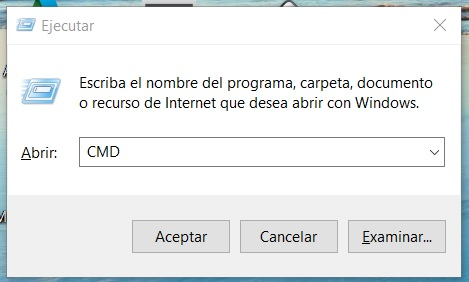
\includegraphics[width=0.5\textwidth]{img/Ejecutar.jpg}
\end{center}

Después de abrir la terminal, debemos verificar que la ruta que nos muestra terminal sea la misma en la que se encuentran los archivos del programa, en caso contrario se puede usar el comando ``cd nombre\_de\_carpeta'' para avanzar a una carpeta o ``cd ..'' para retroceder en la ruta.

    \begin{center}
    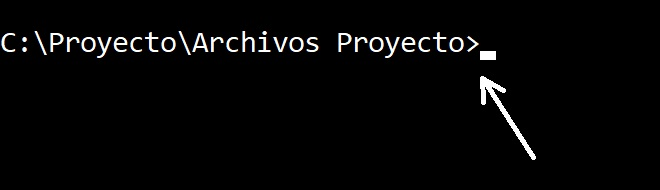
\includegraphics[width = 0.49\textwidth]{img/Ruta Archivos CMD.jpg}
    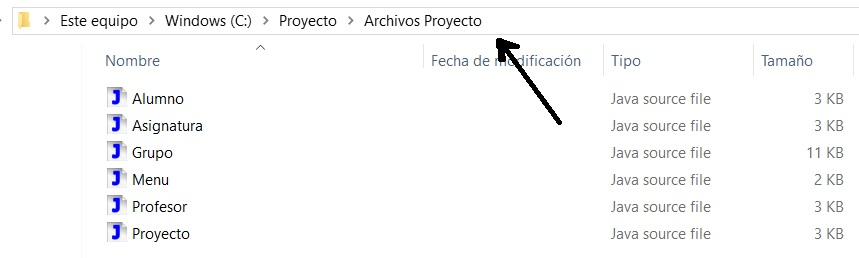
\includegraphics[width = 0.49\textwidth]{img/Ruta Archivos.jpg}
    \end{center}

Una vez situado en la ruta adecuada, basta con teclear ``javac Proyecto.java'', eso hará que el programa compile.

\begin{center}
    \includegraphics[width=0.7\textwidth]{img/Compilación.jpg}
\end{center}

Después de haber tecleado ese comando se debe escribir ``java Proyecto'' para poder ejecutar el programa.

\begin{center}
    \includegraphics[width=0.7\textwidth]{img/Ejecución.jpg}
\end{center}

\subsection*{Registrar Alumno}

Para acceder a esta opción desde el menú principal es necesario escribir ``1'' y presionar ``enter'' con esto se accede a la opción de registro de alumnos.

\begin{center}
    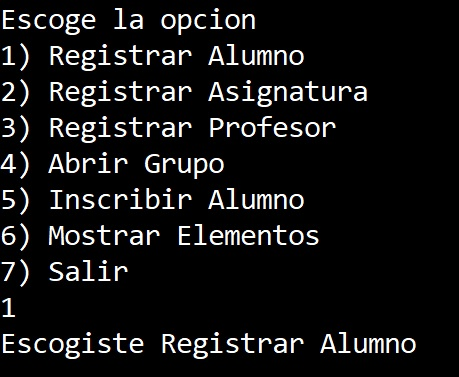
\includegraphics[width=0.7\textwidth]{img/Opcion 1 P1.jpg}
\end{center}

\newpage
Después de haber tecleado ``enter'' mostrará un mensaje en el que debe ingresar la cantidad de alumnos que desea registrar, después deberá ingresar los datos de cada uno de los alumnos, comenzando por nombre, semestre y número de cuenta. Una vez haya terminando de asignar los datos, lo regresará al menu principal.

\begin{center}
    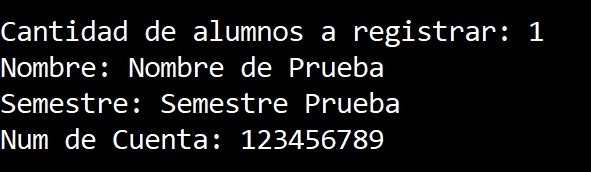
\includegraphics[width=0.7\textwidth]{img/Opcion 1 P2.jpg}
\end{center}

%----------------------------------------------------------------------
\subsection*{Registrar Asignatura}
Para acceder a esta opción es necesario teclear ``2'' desde el menu principal y luego presionar ``enter'' consecuentemente se tiene acceso a el registro de asignaturas.

\begin{center}
    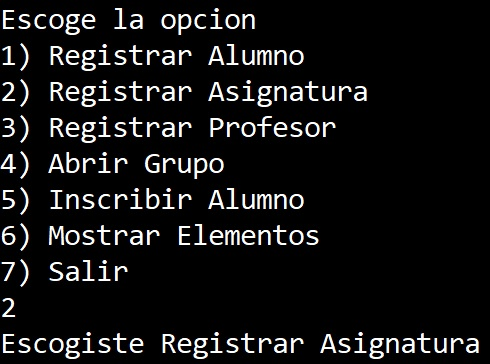
\includegraphics[width=0.7\textwidth]{img/Opcion 2 P1.jpg}
\end{center}

\newpage
Una vez seleccionada la opción mostrará un mensaje en el que debe colocar los datos acerca de las asignaturas que desea registrar.

\begin{center}
    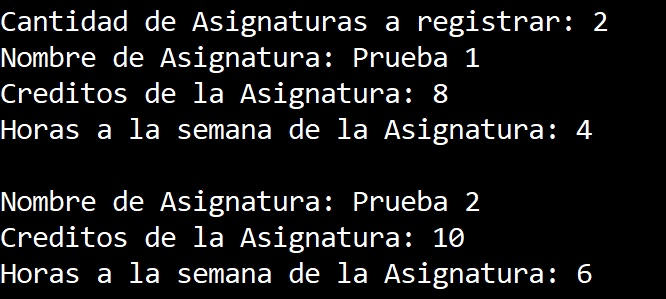
\includegraphics[width=0.7\textwidth]{img/Opcion 2 P2.jpg}
\end{center}

%----------------------------------------------------------------------
\subsection*{Registrar Profesor}
Para acceder a esta opción es irremplazable teclear ``3'' desde el menu principal y luego presionar ``enter'' después de realizar estas acciones se tiene acceso al registro de profesores.

\begin{center}
    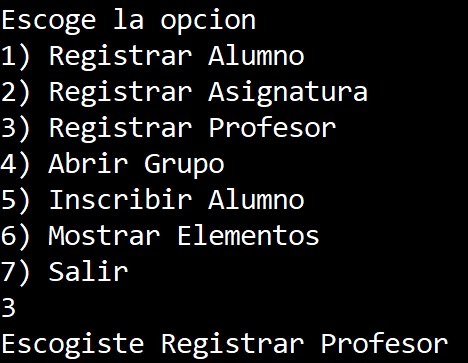
\includegraphics[width=0.7\textwidth]{img/Opcion 3 P1.jpg}
\end{center}

\newpage
Al acceder al registro de profesores en primer lugar imprimirá un mensaje en pantalla el cual debe contestar con la cantidad de profesores que quiere registrar, seguido de haber ingresado la cantidad comenzará a pedir los datos para los profesores.

\begin{center}
    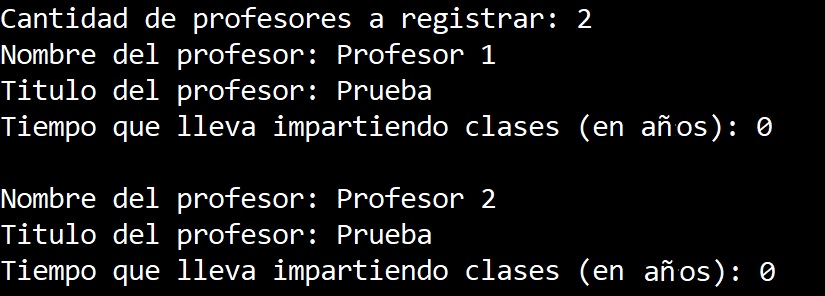
\includegraphics[width=0.7\textwidth]{img/Opcion 3 P2.jpg}
\end{center}

%----------------------------------------------------------------------
\subsection*{Abrir Grupo}
Para tener acceso a esta opción debe teclear ``4'' desde el menu principal y luego presionar ``enter'' cuando se concluyen las dos acciones anteriores tendrá acceso a la abertura de grupos.

\begin{center}
    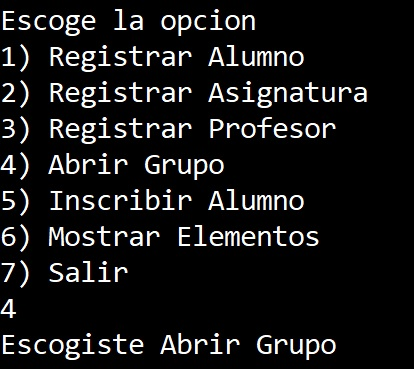
\includegraphics[width=0.7\textwidth]{img/Opcion 4 P1.jpg}
\end{center}

\newpage
Una vez dentro de la opción lo primero que verá es una lista de los profesores y de las asignaturas registradas anteriormente, en primer lugar deberá escribir el NOMBRE de la asignatura de la cual quiere abrir un nuevo grupo, seguido debe escribir el NOMBRE del profesor que quiere asignar a este grupo, en último lugar deberá asignar una clave única al nuevo grupo. En caso de intruducir una clave de grupo que ya se haya ingresado anteriormente deberá ingresar una clave válida. Después de realizar todos estos pasos habrá abierto un grupo nuevo.

\begin{center}
    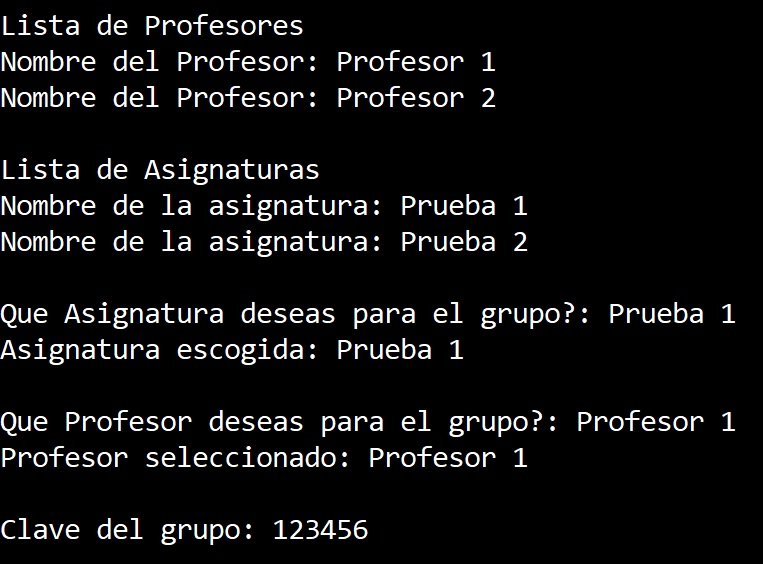
\includegraphics[width=0.7\textwidth]{img/Opcion 4 P2.jpg}
\end{center}


\newpage
%----------------------------------------------------------------------
\subsection*{Inscribir Alumno}
Para inscribir un alumno a un grupo es necesario escribir el número ``5'' y después teclear ``enter'', una vez realizados estos dos pasos se tendrá al acceso de inscripción de alumnos.

\begin{center}
    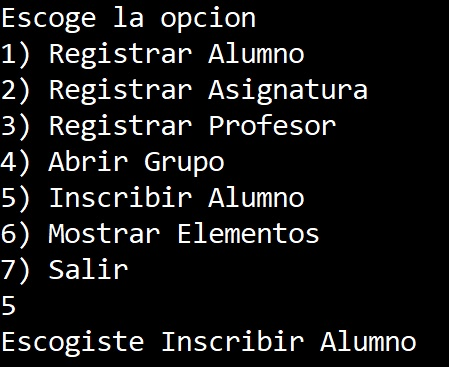
\includegraphics[width=0.7\textwidth]{img/Opcion 5 P1.jpg}
\end{center}

Cuando se accede lo primero que verá serán las claves de los grupos creados además verá nombre y número de cuenta de todos los alumnos registrados, para inscribir un alumno a un grupo en primer lugar deberá escribir la clave del grupo al que quiere inscribirlo, después deberá ingresar el número de cuenta del alumno que desea registrar, cuando los datos son ingresados correctamente el alumno quedará inscrito al grupo.

\begin{center}
    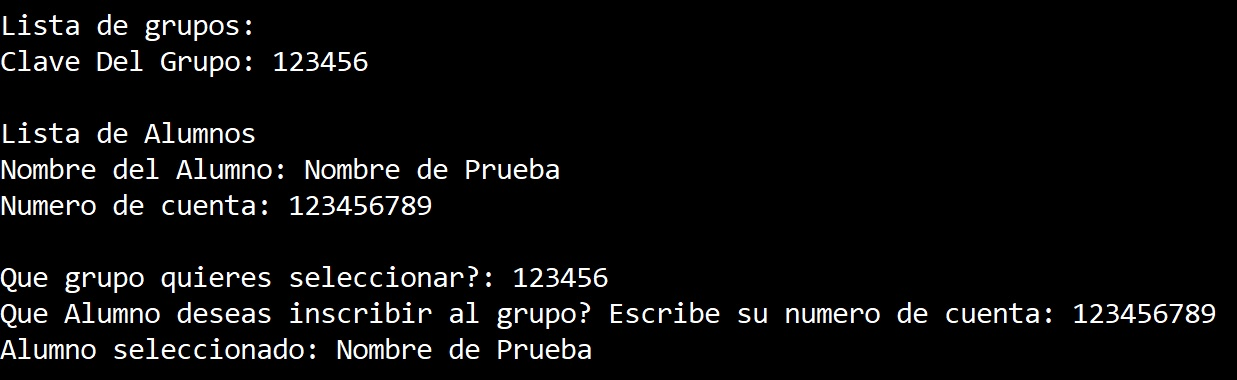
\includegraphics[width=1\textwidth]{img/Opcion 5 P2.jpg}
\end{center}


\newpage
%-------------------------------------------------------------------
\subsection*{Mostrar Elementos}
Para mostrar todos los registros hechos debes teclear ``6'' y presionar ``enter'', cuando se realizan estos pasos exitosamente desplegará otro menú con las opciones que puede mostrar el programa.

\begin{center}
    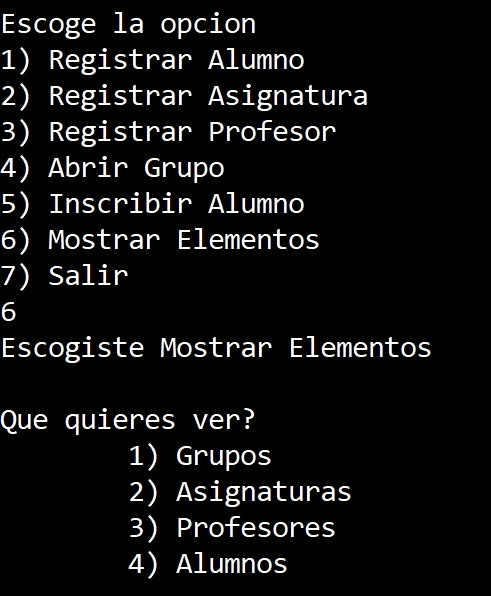
\includegraphics[width=0.7\textwidth]{img/Opcion 6 P1.jpg}
\end{center}

\newpage
\hspace{1cm} \textbf{Mostrar Grupos}

Para poder visualizar todos los grupos creados debe teclear el número ``1'' seguido de ``enter''. 

\begin{center}
    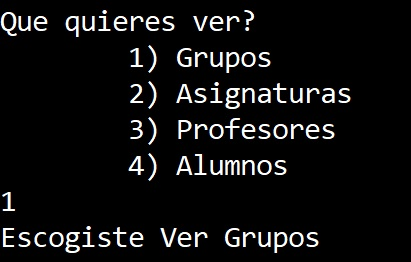
\includegraphics[width=0.8\textwidth]{img/Opcion 6 P2_1.jpg}
\end{center}

Cuando se realizaron con éxito los pasos anteriores el programa mostrará una lista de todos los grupos creados, con el nombre de la asignatura, nombre del profesor y clave de la asignatura. En caso de que en algún grupo ya haya inscritos mostrará la clave del grupo y una lista de todos los alumnos inscritos en el, en caso de no haber grupos con alumnos inscritos sólo mostrará los nombres de asignatura, profesor y la clave de los grupos creados.

\begin{center}
    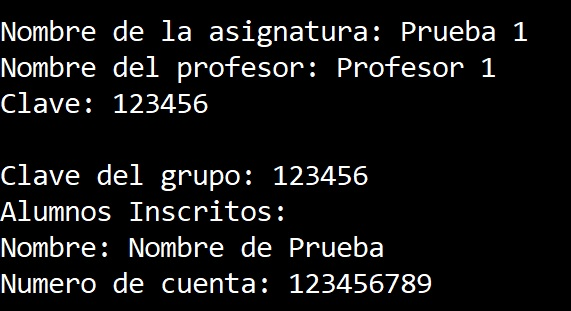
\includegraphics[width=0.8\textwidth]{img/Opcion 6 P2_1_1.jpg}
\end{center}

\newpage
\hspace{1cm} \textbf{Mostrar Asignaturas}

Para poder visualizar todos los grupos creados debe teclear el número ``2'' seguido de ``enter''. 

\begin{center}
    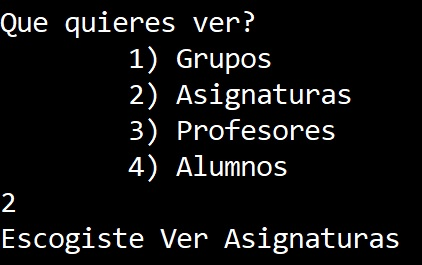
\includegraphics[width=0.8\textwidth]{img/Opcion 6 P2_2.jpg}
\end{center}

Cuando se accede a ver las asignaturas registradas podrá ver los datos que ha asignado a todas las asignaturas que ha registrado anteriormente y finalmente mostrará un mensaje con el total de asignaturas registradas, en caso de no haberlas el programa solo dirá que accedio a ver las asignaturas, sin embargo; el contenido estará vacío.

\begin{center}
    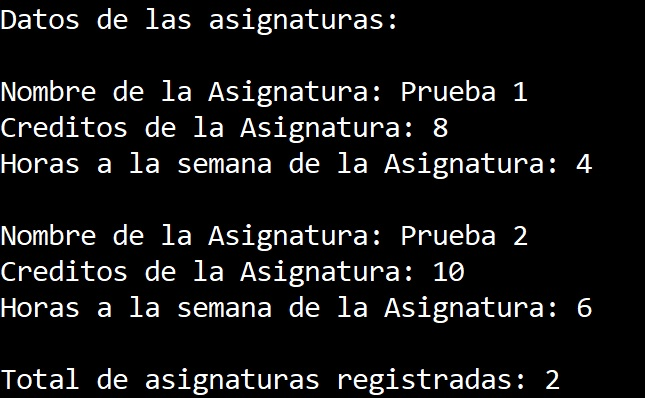
\includegraphics[width=0.8\textwidth]{img/Opcion 6 P2_2_1.jpg}
\end{center}

\newpage
\hspace{1cm} \textbf{Mostrar Profesores}

Para poder visualizar todos los grupos creados debe teclear el número ``3'' seguido de ``enter''. 

\begin{center}
    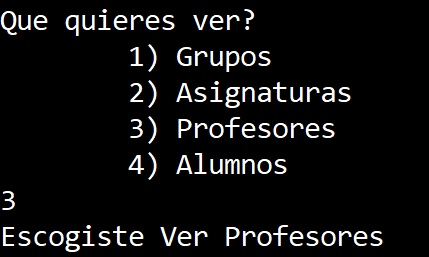
\includegraphics[width=0.8\textwidth]{img/Opcion 6 P2_3.jpg}
\end{center}

Después de tener acceso a la visualización de profesores el programa mostrará una lista en la que estarán todos los profesores registrados con sus datos asignados anteriormente y finalmente mostrará el total de profesores registrados.

\begin{center}
    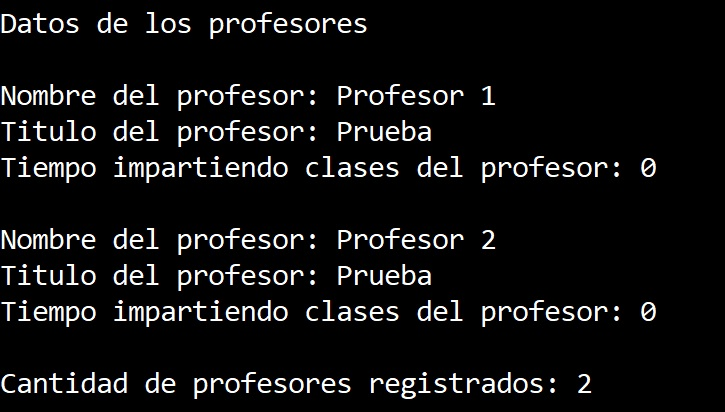
\includegraphics[width=0.8\textwidth]{img/Opcion 6 P2_3_1.jpg}
\end{center}

\newpage
\hspace{1cm} \textbf{Mostrar Alumnos}

Para ver los datos de todos los alumnos registrados debes presionar el número ``4'' y después la tecla ``enter''. 

\begin{center}
    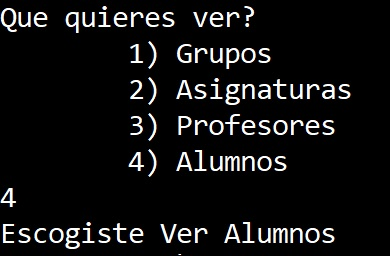
\includegraphics[width=0.8\textwidth]{img/Opcion 6 P2_4.jpg}
\end{center}

Cuando se completan con exito los pasos anteriores, podrá ver en la pantalla los datos asignados a todos los alumnos registrados, para finalizar con la cantidad total de alumnos registrados.

\begin{center}
    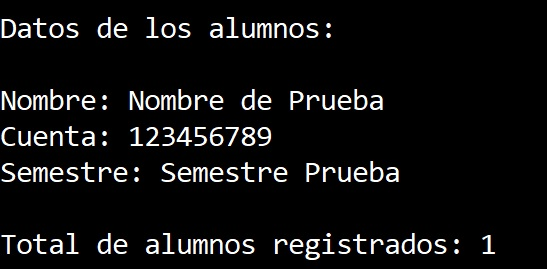
\includegraphics[width=0.8\textwidth]{img/Opcion 6 P2_4_1.jpg}
\end{center}


\newpage
%----------------------------------------------------------------------
\section*{Advertencias de uso}
\begin{enumerate}
    \item En el menú principal sólo se pueden acceder a las opciones mediante números enteros, cualquier otro tipo de entrada causará error en el programa y se dejará de ejecutar.
    \item La forma correcta de salir del programa es teclear y aceptar la opción ``7'' en caso contrario entrará a una opción del menú o mandará un mensaje diciendo que la opción seleccionada es incorrecta.
    \item En la opción de registrar alumno el número de cuenta sólo debe contener números, en caso de contener algún otro carácter causará un error en el programa.
    \item En la opción de registar asignatura el número de créditos y de horas a la semana deben ser números enteros, en caso de contener decimales o algún carácter causará un error en el programa.
    \item En la opción de registar profesor el tiempo que lleva impartiendo clases debe ser un número entero, en caso de no ser así habrá un error y se cerrará el programa.
    \item En la opción de abrir un nuevo grupo debe estar completamente convencido que anteriormente ha registrado al menos una asignatura y al menos un profesor, de lo contrario no podrá salir de la opción y deberá cerrar el programa por lo que tendrá que ejecutarlo todo desde el inicio.
    \item En la opción de Inscribir alumno, debe asegurarse que anteriormente se ha creado al menos un grupo y hay al menos un alumno registrado, de lo contrario entrará a la inscripción pero no podrá salir al menos que cierre el programa, y para volver a acceder a el, tendrá que ejecutar el programa desde el inicio.
    \item En la opción de mostrar elementos el segundo menú que aparece en pantalla deberá ser contestado con un número entero que se encuentre en las opciones mostradas en pantalla, en caso de ser un número entero pero no incluido en las opciones mandará un mensaje de error y lo devolverá al menú principal, en caso de ser otro tipo de dato causará un error en el programa y tendrá que ejecutar todo desde el inicio.
\end{enumerate}

%----------------------------------------------------------------------

\end{document}
